\documentclass{article}
% 11-785 Project Proposal Template
% https://www.overleaf.com/latex/templates/11-785-project-proposal-template/gvfmxtrwcttd
\usepackage{11785_project,times}
\usepackage{hyperref}
\usepackage{url}
\usepackage{graphicx}

\graphicspath{ {./img}}

\title{COMP590--171 Project Proposal: Refraction Networking}

\author{Dohhyun Kim, Harin Lim, Jesse Wei, Daniel Xie, Matseoi Zau}

\date{April 4, 2024}

\begin{document}

\maketitle

\section{Refraction networking introduction}

Refraction networking (RN) is a scheme for evading censorship technology, such as website blacklists enforced by governments, with the help of an ISP partner. Specifically, in refraction networking (also called ``decoy routing''), the user requests a blocked site, but the RN protocol actually requests a reachable site with some encrypted header information. The censor accepts the request that seems to be legitimate, but the ISP partner reads the header information and ``refracts'' the request to the blocked site that the user originally requested.

\begin{figure}[h]
    \centering
    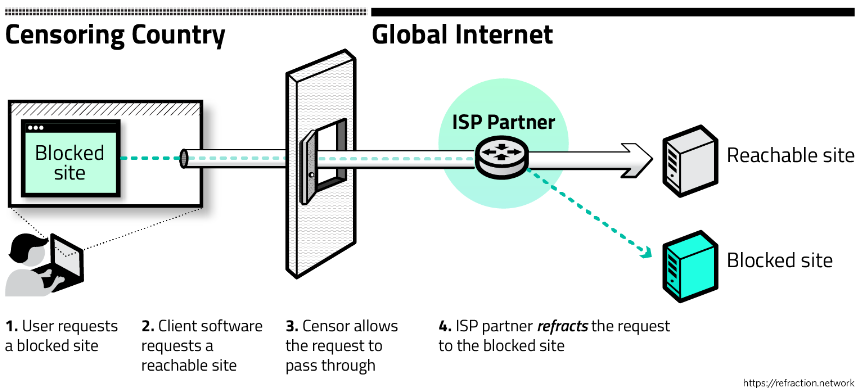
\includegraphics[width=0.8\textwidth]{refraction_networking}
    % TODO: make this not show up as [ref]
    % Note that adding author as "Refraction Network Team" makes the reference [team]
    \caption{Refraction networking \cite{refraction_network}}
\end{figure}

The specific RN protocol we will reimplement for our project is TapDance \cite{tapdance}.

\section{Reimplementation of TapDance}

Our project is to reimplement the TapDance protocol. Specifically, we will simulate censoring a website and bypassing the filter via a client that uses TapDance to request the blocked website and a simulated ISP that refracts the request to the blocked website. We will run the client and server code on different machines with different IP addresses. Finally, we will test out some attacks against TapDance mentioned in the paper to check their viability.

The above will be our artifacts (specifically, code for a TapDance client and server and a simulated ISP).

\section{Schedule}

\begin{center}
\begin{tabular}{|c|c|}
    \hline
    Deadline & Task\\
    \hline
    4/10 & Client, server, ISP (simulated), and website censoring code \\
    \hline
    4/10 & TapDance cryptographic protocols (ECDH, Elligator 2 over Curve25519, etc.) \\
    \hline
    4/21 & TapDance server refraction\\
    \hline
    4/25 & Test attacks against TapDance\\
    \hline
    4/28 & Presentation\\
    \hline
    5/2 & Paper\\
    \hline
\end{tabular}
\end{center}

\section{Team member responsibilities}

Daniel and Matseoi will work on the TapDance cryptographic protocols.

Dohhyun, Harin, and Jesse will work on the client, server, and simulated ISP.

After this is done, the entire team will work on experimenting with attacks against TapDance and writing the presentation and final report.

\newpage
\printbibliography

\end{document}
